%----------------------------------------------------------------------------------------
%	PACKAGES AND OTHER DOCUMENT CONFIGURATIONS
%----------------------------------------------------------------------------------------
\documentclass[a4paper,11pt]{article}
\usepackage[a4paper,textwidth=140mm,textheight=245mm]{geometry}
\usepackage[utf8]{inputenc}
\usepackage{listings}
\usepackage{graphicx}
\usepackage{pstricks}
\usepackage{tikz}
\usepackage{float}
\usepackage{mathtools}
\usepackage{subscript}
\makeatletter
\renewcommand{\section}{\@startsection
   {section}%                         name
   {1}%                               level
   {0mm}%                             indent
   {-1.5\baselineskip}%               space above header
   {0.5\baselineskip}%                space under header
   {\sffamily\bfseries\upshape\normalsize}}% style
   
\renewcommand{\subsection}{\@startsection
   {subsection}%                      name
   {2}%                               level
   {0mm}%                             indent
   {-0.75\baselineskip}%              space above header
   {0.25\baselineskip}%               space under header
   {\rmfamily\normalfont\slshape\normalsize}}% style
\renewcommand{\subsubsection}{\@startsection
   {subsubsection}%                    name
   {3}%                               level
   {0mm}%                             indent
   {-0.75\baselineskip}%              space above header
   {0.25\baselineskip}%               space under header
   {\rmfamily\normalfont\slshape\normalsize}}% style
\makeatother
\begin{document}
\begin{titlepage}
\title{TSKS10 sammanfattning}
\author{Martin Söderén\\ marso329@student.liu.se\\900929-1098}
\date{\today}
\maketitle




\vfill % Fill the rest of the page with whitespace

\thispagestyle{empty}

\end{titlepage}

\newpage
\tableofcontents	%Innehållsförteckning

\newpage

\section{Trigonometric identities}
$$sin(u)sin(v)=\frac{1}{2} [cos(u-v)-cos(u+v)]$$

$$cos(u)cos(v)=\frac{1}{2} [cos(u-v)+cos(u+v)]$$

$$sin(u)cos(v)=\frac{1}{2} [sin(u+v)+sin(u-v)]$$

$$cos(u)sin(v)=\frac{1}{2} [sin(u+v)-sin(u-v)]$$
\section{Digital kommunikationslänk}
source coding-channel coding(error protection)-digital modulation-channel-syncronization och equalization och demodulation-channel decoding-decompression

\section{I/Q representation}
$$ x(t)=x_I(t)cos(2\pi f_ct)-x*Q(t)sin(2\pi f_c t)$$
$$x_I(t)=\mathcal{H}_{B/2}^{LP} \{ 2x(t)cos(2\pi f_c t)\}$$
$$x_Q(t)=-\mathcal{H}_{B/2}^{LP} \{ 2x(t)sin(2\pi f_c t)\}$$
$$\bar{x}(t)=\sqrt{x_I^2(t)+x_Q^2(t)}$$
$\phi_x(t)$ is chosen to satisfy :
$$x_I(t)=\bar{x}(t)cos(\phi_x(t)) $$
$$x_Q(t)=\bar{x}(t)sin(\phi_x(t)) $$

\section{dimensionality pam}
Dimensionality=length of signal * bandwidth

\section{Direct modulation}
Transforming a narrowband signal to a band-limited signal with $f_c$=0.
$$y(t)=\mathcal{H}_{B}^{LP}\{ 2x(t)cos(2\pi(f_c -\frac{B}{2})t) \}$$
Inverse tranformation:
$$x(t)=\mathcal{H}_{f_c-B/2,f_c+B/2}^{BP}\{ 2y(t)cos(2\pi(f_c -\frac{B}{2})t) \}$$

\section{Small time delay}
If a signal is time shifted $\tau$ and $\tau<1/B$ then:
$$x(t-\tau)=\bar{x}(t)cos(2\pi f_c t+\phi_x(t)-2\pi f_c \tau)$$
 
 \section{Dimensionality in time-frequency space}
 $$dimensionality=2BT$$
 Where B is the bandwidth and T is the duration of the signal.
 
 \section{sample a truncated signal}
 By trunacting a signal its spectrum will be wider. Let assume that a signal with bandwidth $[-B,B] Hz$ is truncated into $[-T/2,T/2]$ then the new bandwidth of the signal will be $[-B-\frac{1}{T},B+\frac{1}{T}]$
 
 \section{Sample theorem}
 If a signal has bandwidth B then it must be sampled with $f\geq 2B$
 
 \section{Undersampling}
 You can sample a bandpass signal which $f_c\ne0$ with a sample rate lower than the one required by the nyquist criterion. If the signal is present in $[f_l,f_h]$ then
 the signal can be sampled with $f_s$ from the formula
 $$\frac{2f_h}{n}\leq f_s \leq \frac{2f_l}{n-1}$$
 for any integer n that satisfies:
 $$1\leq n \leq \frac{f_h}{f_h+f_l}$$
 
 \section{Teorifrågor}
För en vågformskanal, så är datatakten (i bitar per sekund) alltid lika med kanalens
bandbredd i Hertz. Svar: falskt relationen mellan datatakt och bandbredd är det som kallas spektraleffektivitet
\newline
\newline
En kabel har alltid en reellvärd karaktäristisk impedans.
svar: Nej, den kan ha imaginaär impedans.
\newline
\newline
Vilken kabel som helst kan få en reellvärd karaktäristisk impedans, bara man kop-
plar den till en lämpligt anpassad last.
svar: Nej impedans beror inte på lasten. 
\newline
\newline
Hammingkoden har en datatekt som är 3/7. Svar: falskt den är 4/7
\newline
\newline
En suddkanal (binary erasure channel) kan aldrig ha en kapacitet på mer än 1.5
bitar per kanalanvändning (1.5 bits per channel use). Svar: sant, den kan inte har mer än 1 bit per channel
\newline
\newline
är signalen:
$$x(t)=\int_{-\infty}^{\infty}sinc(t-\tau)e^{-|\tau|/7}$$
svar: ja då detta är en faltning med sinc så ger detta multiplicering med en rektangelfunktion i frekvensdomänen.
\newline
\newline
Vad innebär det att en signal är strikt bandbegränsad? Approximativt bandbegränsad? 
svar: Strikt bandbegränsad betyder att den har sin energi fördelad på ett ändligt frekvensintervall.  Approximativt innebär att om energin är under en viss nivå över en frekvensgräns så tar man bort dessa frekvenser för att få en bandbegränsad signal(gissning)
\newline
\newline
Vad innebär det att en signal är strikt tidsbegränsad? Approximativt tidsbegränsad?
svar: Att dess amplitud är skild från noll under ändlig tid. Approximativt innebär att dess amplitud nästan är skild från noll under ändlig tid och man kan ta bort dessa amplituder.
\newline
\newline
Definiera energin av en signal.
$$E_s=\int_{-\infty}^{\infty}{|x(t)|^2dt}$$
\newline
\newline
Definiera Fouriertransformen X(f) av en tidskontinuerlig signal x(t), samt dess invers.
svar: $$X(f)=\int_{-\infty}^{\infty}x(t)e^{-it2\pi f}$$
$$f(t)=\frac{1}{2 \pi}\int_{-\infty}^{\infty}X(f)e^{it2\pi f}$$
\newline
\newline
Definiera Fouriertransformen X[F] av en tidsdiskret signal x[n], samt dess invers.
$$X[f]=\sum_{-\infty}^{\infty}x[n]e^{i2\pi f n}$$
$$x[n]=\frac{1}{2\pi}\int_{-\infty}^{\infty}X[f]e^{i2\pi f n}$$
\newline
\newline
Ge två exempel på kvantitativa bandbredds-mått.
svar: Beskriver kapaciteten på en kommunikationskanal. 
\newline
\newline
Om en signal x(t) trunkeras till ett ändligt intervall [-T/2,T/2], vad händer då med X(f)? Rita en figur. Svar: De högre frekvenserna i transformen försvinner och X(f) blir ojämnare. 
\newline
\newline
Formulera samplingsteoremet, och ge en formel för rekonstruktion.
Svar: En signal med bandbredd b måste samplas med minst frekvensen 2b för att garantera perfekt rekonstruktion. 
$$x(t)=\sum_{-\infty}^{\infty}x(nT)sinc(\frac{t-nT}{T})$$
\newline
\newline
Vad är dimensionalitet?  Vilken dimensionalitet har en signal som bor i [-T/2,T/2]x[B,B] 
och varför? Svar: Hur många variabler som behövs för att beskriva signalen. Signalen är endimensionel då den kan beskrivas i båda domänerna med en variabel t eller f.
\newline
\newline
Vad är skillnaden mellan en lågpass- (basband) signal och en smalbandig 
(passband/bandpass) signal? svar: En lågpass signal har 0 Hz som lägre gränsfrekvens.
\newline
\newline
Hur fungerar direkt demodulation (nedblandning)? Rita relevanta diagram.
Svar: man ändrar bärsignalens frekvens. Säg att man har skickat en signal på en högfrekvent frekvens och sedan nedblandar man dig för att sampla den vid en lägre frekvens. 
\newline
\newline
Beskriv hur I/Q modulering/demodulering fungerar och rita ett tillhörande blockdiagram. 
Inkludera alla väsentliga komponenter.
\newline
\centerline{
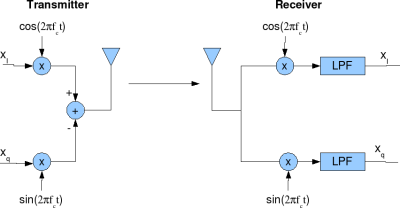
\includegraphics[scale=0.7]{IQ}
}
\newline
\newline
Definiera envelopp och fas för en smalbandig signal.
Svar:
$$A(t)=\sqrt{I^2(t)+ Q^2(t)}$$
$$\phi(t)=tan^{-1}(\frac{Q(t)}{I(t)})$$
\newline
\newline
Vad har en liten tidsfördröjning för effekt på I och Q komponenterna för en smalbandig 
signal?  Beskriv eller härled relevanta samband.
\newline
\newline
Vad är nyttan med I/Q representationen och varför används den i praktiken?
svar: man vet om frekvensen hos en representerad signal är positiv eller negativ. Man samplar signal på dess toppar och får bättre data. 
\newline
\newline
Beskriv pulsamplitudmodulering i tidsdomänen. Rita relevanta figurer.
Man samplar amplituden i den signal
\newline
\newline
Beskriv pulsamplitudmodulering i frekvensdomänen.  Rita relevanta figurer.
\newline
\newline
Ge Poisson's summationsformel och illustrera med en figur vad som händer i 
frekvensdomänen.
\newline
\newline
Vad är vikning? När uppstår vikning och hur kan det undvikas?
Man samplar med för låg frekvens så signalen överlappar. Öka samplingsafrekvensen.
\newline
\newline
Hur snabbt måste man sampla för att undvika vikning och varför?
Dubbla bandbredden på grund av samplinsteoremet. 
\newline
\newline
Beskriv vad ideal rekonstruktion är.
Svar: Man förlorar ingen information jämfört med signalen som först dekonstruerades.
\newline
\newline
Rita en enkel modell för digital signalbehandling av analoga signaler.  Inkludera alla 
väsentliga komponenter.
Rita en adc.
\newline
\newline
Rita en enkel modell för en kommunikationslänk där pulsamplitudmodulering används.  
Inkludera alla väsentliga komponenter.
\newline
\centerline{
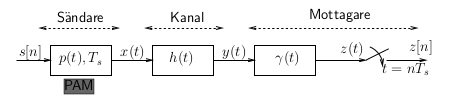
\includegraphics[scale=0.7]{pam}
}
\newline
\newline
Formulera Nyquist-kriteriet för pulsamplitudmodulering, i tidsdomänen. 
$$1/T_s>2B$$
\newline
\newline
Formulera Nyquist-kriteriet för pulsamplitudmodulering, i frekvensdomänen.
$$f>2B$$
\newline
\newline
Beskriv hur en FFT kan användas för att skatta spektrum av en tidskontinuerlig signal.
\newline
\newline
Vad innebär att en signal är slumpmässig?  
svar: brus
\newline
\newline
Vad är en vit slumpmässig signal? 
Har konstant spektral energi
\newline
\newline
Vad är brus?
en slumpmässig signal
\newline
\newline
Beskriv termiskt brus, var/när uppkommer det och varför.
Elektronsikt brus som uppkommer på grund av att elektroner blir agiterade. 
\newline
\newline
Beskriv kvantiseringsbrus, var/när uppkommer det och varför.
När man samplar en signal får man kvantiseringsbrus. Detta kan man motverka genom att öka antalet bitar man använder för varje sample. 
\newline
\newline
Vad innebär det att brus är Gaussiskt? Varför är detta ofta en bra och vanlig modell?
bruset är normalfördelat övar alla frekvenser run en bestämd frekvens.
\newline
\newline
Definiera signal-till-brus-förhållande (SNR) i en signal. Vad är betydelsen av SNR?
$$SNR=\frac{P_{signal}}{P_{noise}}$$ där p är power. SNR står för signal-noise-ratio
\newline
\newline
Beskriv en tumregel för SNR i en likformigt kvantiserad signal. 
varje extra bit bidrar till 6db ökad SNR
\newline
\newline
Beskriv en enkel modell för tidsfördröjnings-skattningsproblemet.
\newline
\newline
Beskriv hur skattning av tidsfördröjningar med hjälp av korrelation fungerar.
\newline
\newline
Vad är en mångtydighetsfunktion? Hur är den definierad? Varför är den relevant för 
skattningar av tidsfördröjningar?
\newline
\newline
Vilka egenskaper har en signal som är väl lämpad till skattningar av tidsfördröjningar, och 
varför?
\newline
\newline
Ge två exempel på signaler som typiskt används för att skatta tidsfördröjningar.
\newline
\newline
Beskriv två tillämpningar av tidsfördröjnings-skattningar.
\newline
\newline
Vad är en spöktopp och varför uppkommer en sådan?
\newline
\newline
Vad är relationen mellan nogrannhet i skattningar av tidsfördröjningar och bandbredden på 
signalen som används? Varur kommer denna relation?
\newline
\newline
Vad är en chirp-vågform?  Vad har den för egenskaper?
\newline
\newline
Vad innebär det att en vågform har konstant envelopp?  Är detta önskvärt eller inte, och i så 
fall varför (eller varför inte)?
\newline
\newline
Vad är entropi?
\newline
\newline
Vad är en binär källa?  Hur stor och hur liten entropi kan en binär källa ha och varför?
\newline
\newline
Vad har en binär källa att göra med att singla slant?
\newline
\newline
Om ett mynt med p=0.1 kastas 100 gånger, vad kan vi förvänta oss att se?
\newline
\newline
Vad är en typisk sträng?
\newline
\newline
Definiera och rita den binära entropifunktionen. Vad är den operativa betydelsen av denna 
funktion? 
\newline
\newline
Varför är entropi ett mått på komprimerbarhet? 
\newline
\newline
Varför är entropi ett mått på informationsinnehåll?
\newline
\newline
Vad är entropin för en M-värd källa? Hur relaterar en sådan källa till ett tärningskast?
\newline
\newline
Beskriv hur skurlängdskodning fungerar. När förväntas sådan kodning fungera bra? 
\newline
\newline
Beskriv hur Huffmankodning fungerar.
\newline
\newline
Vad kan man säga om relationen mellan längden på kodorden i en Huffmankod och entropin
hos källan som ska komprimeras?
\newline
\newline
Vad är förlustfri komprimering? Ge ett exempel.
\newline
\newline
Vad är ej förlustfri komprimering? Ge två exempel.
\newline
\newline
Nämn två tillämpningar av källkodning.
\newline
\newline
Formulera 
källkodningssatsen
, för förlustfri komprimering och en M-värd källa.
\newline
\newline
Vad innebär det att en datamängd innehåller redundans?  Ge exempel på redundans i skriven
text på svenska.
\newline
\newline
Varför är det typiskt önskvärt att ta bort redundans med hjälp av datakompression?
\newline
\newline
Varför är det typiskt önskvärt att tillsätta redundans med hjälp av kanalkodning?
\newline
\newline
Om ett meddelande (t.ex. text på svenska) redan innehåller redundans, varför är det då 
meningsfull att först ta bort denna redundans med hjälp av datakompression och sedan 
tillsätta annan redundans med hjälp av kanalkodning?
\newline
\newline
Vad är en binär kanal?  Rita en figur.
\newline
\newline
Vad är en binärsymmetrisk kanal? Rita en figur. Vad har en sådan kanal för kapacitet?
\newline
\newline
Vad är en suddkanal? Rita en figur. Vad har en sådan kanal för kapacitet?
\newline
\newline
Vad är en kodbok (för kanalkodning)? Definiera dess takt och min-avstånd. Beskriv hur 
takten relaterar till antal kodord och kodordens längd.
\newline
\newline
Vad är en avkodare? Vad arbetar avkodaren efter för princip?
\newline
\newline
Vad är felsannolikhet?
\newline
\newline
Om en kodbok har minavståndet d, hur många fel (antal felaktigt mottagna binära siffror) 
kan denna rätta och varför?
\newline
\newline
Vad repetitionskodning? Vad har en repetitionskod för takt?  Vad har den för minavstånd? Är
en repetitionskod bra eller dålig?
\newline
\newline
Vad är en (7,4)-Hammingkod? Vad har den för takt? Vad har den för minavstånd?  
\newline
\newline
Vad är ömsesidig information? 
\newline
\newline
Vad är kanalkapacitet?
\newline
\newline
Formulera 
kanalkodningssatsen
för en binär-symmetrisk kanal.
\newline
\newline
Nämn någon klass av kanalkoder som används i praktiken och ungefär när den är 
utvecklad/uppfunnen.
\newline
\newline
Vad är en diskret minneslös kanal? Rita en figur.
\newline
\newline
Vad är en additivt-Gaussiskt-brus kanal? Rita en figur.
\newline
\newline
Vad är en vågformskanal? Rita ett blockdiagram.
\newline
\newline
Vad är en LTI-vågformskanal?  Rita ett blockdiagram.
\newline
\newline
Vad är koherenstid för en vågformskanal?
\newline
\newline
Vad är koherensbandbredd för en vågformskanal? Under vilka förutsättningar är denna 
definierad?
\newline
\newline
Vad är "delay spread" för en kanal? Under vilka förutsättningar är denna definierad? Hur 
relaterar "delay spread" till koherensbandbredden?
\newline
\newline
Vad är ett koherensintervall?
\newline
\newline
Vad är en frekvens-flat kanal? 
\newline
\newline
Vad är en frekvens-selektiv kanal?
\newline
\newline
Vad innebär att arbetspunkten för en vågformskanal är i det bandbredds-begränsade 
området?
\newline
\newline
Vad innebär att arbetspunkten för en vågformskanal är i det effekt-begränsade området?
\newline
\newline
Rita upp den fysikaliska modell för en kabel som används i S.I.C.  Beskriv (mycket koncist) 
alla väsentliga komponenter.
\newline
\newline
Vad är karakteristisk impedans hos en kabel?  Vilka parametrar beror den på? 
\newline
\newline
Vad innebär det att en kabel är inkopplad till en anpassad last?
\newline
\newline
Under vilka förutsättningar blir frekvenssvaret H(f) för en kabel (belastad med någon 
impedans Z(f)), konstant med avseende på f?
\newline
\newline
Vad händer om en kabel belastas med en missanpassad last?
\newline
\newline
Hur snabbt kan en signal propagera över en kabel?
\newline
\newline
Beskriv tre huvudsakliga fenomenen som spelar in när en radiosignal breder ut sig över en 
trådlös (markbunden radio) kanal.
\newline
\newline
Vad är sträckdämpning? Varför uppkommer denna?
\newline
\newline
Vad är storskalig fädning/skuggfädning? Varför uppkommer denna?
\newline
\newline
Vad är småskalig fädning? Varför uppkommer denna?
\newline
\newline
Relatera, kvantitativt, koherenstiden för en trådlös kanal till hastigheten hos en rörlig
sändare eller mottagare.
\newline
\newline
Relatera, kvantitativt, koherensbandbredden för en trådlös kanal till hur 
utbredningsmiljön ser ut.
\newline
\newline
Vad är en fädnings-dipp? När och varför uppkommer en sådan?
\newline
\newline
Vad är Rayleigh-fädning? Varför uppkommer denna och när (ge exempel) är den en 
relevant modell? 
\newline
\newline
Var är "single sideband" AM? Rita, i frekvensdomänen, vad som sker vid 
modulering.
\newline
\newline
Vad är "double sideband" AM? Rita, i frekvensdomänen, vad som sker vid 
modulering.
\newline
\newline
Var är analog frekvensmodulation? Beskriv hur det fungerar, med en ekvation.
\newline
\newline
Vad har en digital kommunikationslänk för fördelar över en analog? Vad har den för 
nackdelar?
\newline
\newline
Rita ett blockschema över en digital kommunikationslänk och beskriv (mycket 
koncist) vilken roll de olika komponenterna har.
\newline
\newline
Vad är "channel state information" (CSI)? Hur kan sändare få CSI? Hur kan en 
mottagare få CSI? Vad kan sändaren ha för nytta av CSI? Vad kan mottagaren ha för nytta av
CSI?
\newline
\newline
Hur fungerar digital modulation? Vad är en symbol?  Vad är linjär modulation? Vad 
är olinjär modulation?
\newline
\newline
Vad innebär tids- och frekvens-synkronisering? Varför behövs dessa funktioner och 
hur fungerar
 
\end{document}